\documentclass[pscyr]{hedwork}
\usepackage[russian]{babel}
\usepackage[derivative,root,shortcuts,environments]{hedmaths}

\faculty{Факультет электроники и вычислительной техники}
\department{<<Физика>>}
\subject{Термодинамика и статистическая физика}
\variant{16}
\student[f]{студентка группы Ф-469 \\ Слоква В. И.}
\teacher[m]{профессор, д. физ.-мат. н. \\ Крючков С. В.}

\renewcommand{\labelenumi}{\asbuk{enumi})}
\newcommand{\tpder}[3]{\left(\pder{#1}{#2}\right)_{\!\!#3}}

\makeatletter
  \@addtoreset{equation}{task}
  \renewcommand{\theequation}{\thetask.\arabic{equation}}
\makeatother

\usepackage{graphicx}
\graphicspath{{images/slock_}}

\begin{document}

  \maketitle

  \begin{task}{10 (ТД)}{
    Получите выражение критических параметров \( V_\text{к} \),
    \( p_\text{к} \), \( T_\text{к} \) через константы уравнения состояния,
    предложенного Бертло для описания поведения реальных газов:
    \[
      \left(p + \frac{a}{TV^2}\right)\cdot\Bigl(V - b\Big) = RT.
    \]
  }
  
    В критической точке 
    \( \ds \left(\pder{p}{V}\right)_{\!\! T=T_\text{кр}}\!\!\! = 0 \)
    и \( \ds \left(\ppder{p}{V}\right)_{\!\! T=T_\text{кр}}\!\!\! = 0 \).
    
    Дифференцируем уравнение Бертло:
    \begin{gather*}
      \left[\left(\pder{p}{V}\right)_{\!\! T_\text{кр}} -
        \frac{2a}{T_\text{кр}V_\text{кр}^3}\right]\Big[V_\text{кр} - b\Big]
        + p_\text{кр} + \frac{a}{T_\text{кр}V_\text{кр}^2} = 0. \\
      \left[\left(\ppder{p}{V}\right)_{\!\! T_\text{кр}} +
        \frac{6a}{T_\text{кр}V_\text{кр}^4}\right]\Big[V_\text{кр} - b\Big]
        + 2\cdot\left[\left(\pder{p}{V}\right)_{\!\! T_\text{кр}} -
        \frac{2a}{T_\text{кр}V_\text{кр}^3}\right] = 0.
    \end{gather*}
    
    Отсюда найдем критические параметры, обнуляя производные:
    \begin{gather*}
      \frac{6a}{T_\text{кр}V_\text{кр}^4}\Big[V_\text{кр} - b\Big] =
        \frac{4a}{T_\text{кр}V_\text{кр}^3}, \quad
        3 - 3b / V_\text{кр} = 2, \quad V_\text{кр} = 3b. \\
      -\frac{2a}{T_\text{кр}\,27b^3}2b + p_\text{кр} +
        \frac{a}{T_\text{кр}\,9b^2} = 0, \quad p_\text{кр} =
        \frac{a}{27b^2T_\text{кр}}. \\
      \left(\frac{a}{27b^2T_\text{кр}} + \frac{a}{9b^2T_\text{кр}}\right)2b
        = RT_\text{кр}, \quad
        \frac{8ab}{27b^2T_\text{кр}} = RT_\text{кр}, \quad
        T_\text{кр} = \sqrt{\frac{8a}{27bR}}. \\
      p_\text{кр} = \frac{a}{27b^2}\sqrt{\frac{27bR}{8a}} =
        \sqrt{\frac{aR}{216\,b^3}}.
    \end{gather*}

  \end{task}

  \begin{task}{86 (ТД)}{
    Покажите, что сжатие газа по политропе, идущей на диаграмме \( p \) и
    \( V \) круче адиабаты, сопровождается поглощением тепла.
  }
  
    \begin{figure}[h!]
      \center
      \begin{minipage}{.38\textwidth}
        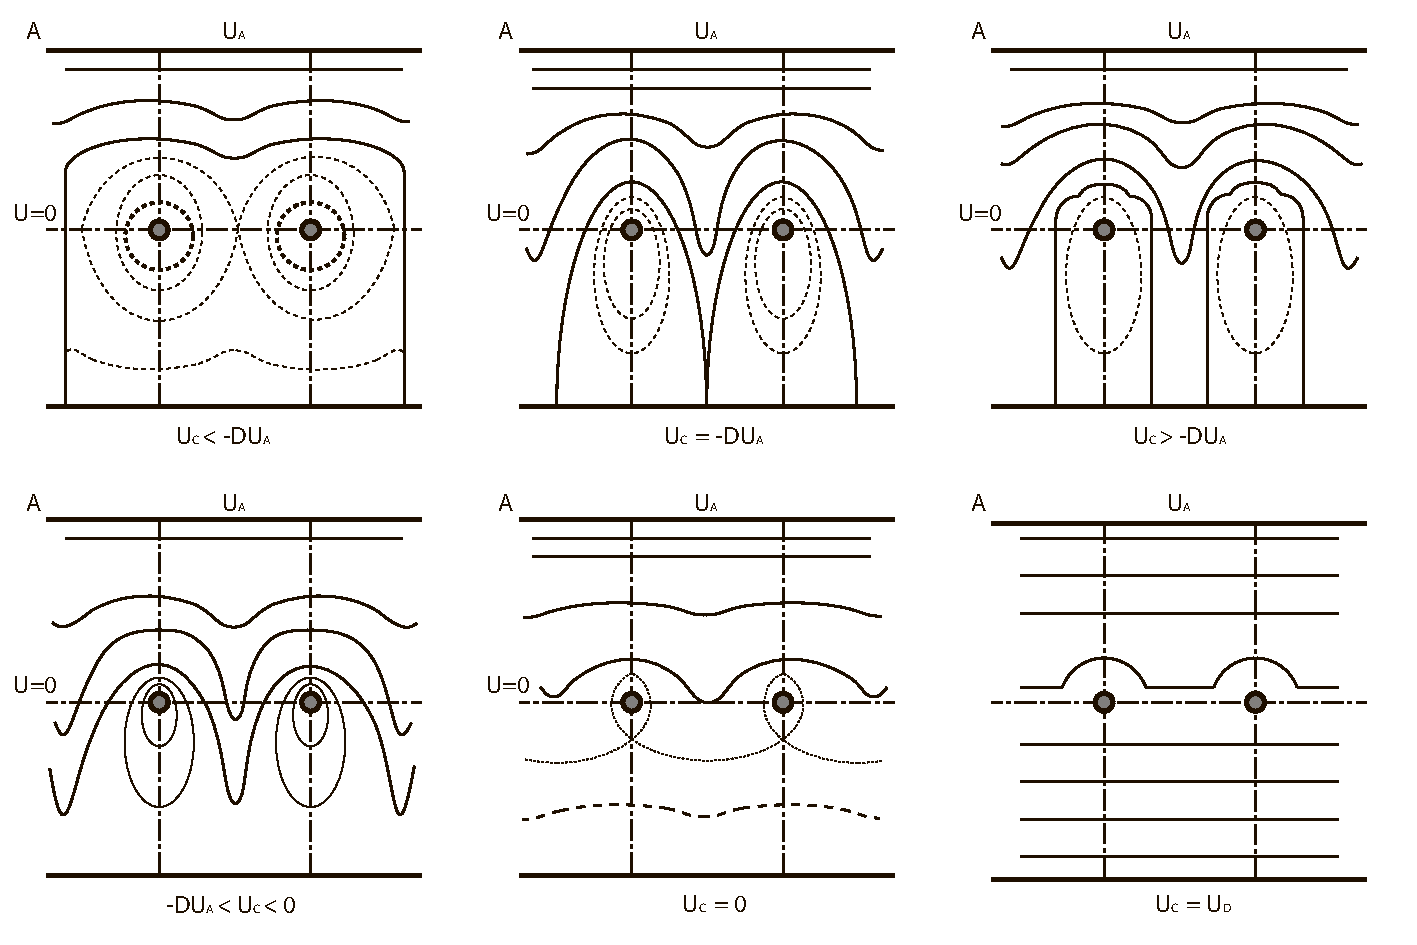
\includegraphics[width=\textwidth]{2}
      \end{minipage} \hfill
      \begin{minipage}{.6\textwidth}
        Первое начало термодинамики:
        \begin{gather*}
          \d Q = dU + \d A, \text{ где } \d A = p\,dV \text{ и } dU =
            C_V\,dT. \\
          \d Q = C_V\,dT + p\,dV.
        \end{gather*}
    
        Связь \( C_V \) с показателем адиабаты:
        \[
          C_V = R / (\gamma - 1).
        \]
        Из уравнения Менделеева-Клапейрона:
        \[
          pV = RT, \quad R\,dT = p\,dV + V\,dp.
        \]
      \end{minipage}
    \end{figure}
    
    Тогда количество теплоты:
    \[
      \d Q = \frac{p\,dV}{\gamma - 1} + \frac{V\,dp}{\gamma - 1} + p\,dV =
        \frac{\gamma}{\gamma - 1}p\,dV + \frac{1}{\gamma - 1}V\,dp.
    \]
    
    Или
    \[
      \frac{\d Q}{dV} = \frac{\gamma p}{\gamma - 1} +
        \frac{V}{\gamma - 1}\der{p}{V}.
    \]
    
    Если процесс адиабатный, то \( \d Q = 0 \) и
    \[
      \der{p}{V} = -\gamma\frac{p}{V}.
    \]
    
    В нашем случае, поскольку политропа идет круче адиабаты,
    \[
      \der{p}{V} < -\gamma\frac{p}{V}.
    \]
    
    И тогда
    \[
      \frac{\d Q}{dV} < \frac{\gamma p}{\gamma - 1} -
        \frac{\gamma p}{\gamma - 1} = 0.
    \]
    
    Так как газ сжимается, то \( dV < 0 \) и, следовательно, \( \d Q > 0 \), то
    есть тепло поступает в систему.
  \end{task}
  
  \begin{task}{127 (ТД)}{
    Определите к.~п.~д. цикла Карно, рабочим веществом в котором является газ
    Ван-дер-Ваальса, и покажите, что он равен к.~п.~д. цикла Карно с идеальным
    газом.
  }
  
    Уравнение Ван-дер-Ваальса относительно давления \( p \):
    \begin{equation}
      p(T, V) = \frac{RT}{V - b} - \frac{a}{V^2}. \label{eq:3.1}
    \end{equation}
  
    Внутренняя энергия газа Ван-дер-Ваальса:
    \begin{equation}
      U(T, V) = C_VT - a / V. \label{eq:3.2}
    \end{equation}
  
    В адиабатическом процессе \( \d Q = dU + \d A = 0 \):
    \begin{equation}
      \left(\pder{U}{T}\right)_V\,dT + \left(\pder{U}{V}\right)_T\,dV +
        p\,dV = 0. \label{eq:3.3}
    \end{equation}
    
    Подставив~\eqref{eq:3.1} и~\eqref{eq:3.2} в~\eqref{eq:3.3}, получим
    \begin{gather*}
      C_V\,dT + \frac{a}{V^2}\,dV + \frac{RT}{V - b}\,dV -
        \frac{a}{V^2}\,dV = 0, \\
      C_V\,dT + \frac{RT}{V - b}\,dV = 0, \quad
        \frac{dT}{T} + \frac{R}{C_V(V - b)}\,dV = 0, \quad
        \frac{dT}{T} + \frac{\gamma - 1}{V - b}\,dV = 0,
    \end{gather*}
    поскольку \( \gamma = C_p / C_V = R / C_V + 1 \). Проинтегрировав, получим
    \[
      0 = \ln T + (\gamma - 1)\ln(V - b) + \const, \text{ или }
        T(V - b)^{\gamma - 1} = \const.
    \]
    
    Таким образом, для адиабатических процессов
    \begin{gather*}
      T_1(V_2 - b)^{\gamma - 1} = T_2(V_3 - b)^{\gamma - 1}, \quad
        T_1(V_1 - b)^{\gamma - 1} = T_2(V_4 - b)^{\gamma - 1}, \\
      \frac{V_2 - b}{V_1 - b} = \frac{V_3 - b}{V_4 - b}.
    \end{gather*}
    
    Подводимое \( Q_1 \) и отводимое \( Q_2 \) количества теплоты:
    \begin{gather*}
      Q_1 = \int\limits_{V_1}^{V_2} p(V, T_1)\,dV + U(V_2, T) - U(V_1, T) =
        \int\limits_{V_1}^{V_2} \frac{RT_1}{V - b}\,dV -
        \int\limits_{V_1}^{V_2} \frac{a}{V^2}\,dV + \\
      + U(V_2, T) - U(V_1, T) = RT_1\ln(V_2 - b) - RT_1\ln(V_1 - b) +
        \frac{a}{V_2} - \frac{a}{V_1} + \\
      + C_VT_1 - \frac{a}{V_2} - C_VT_1 + \frac{a}{V_1} =
        RT_1\ln\frac{V_2 - b}{V_1 - b}.
    \end{gather*}
    
    Аналогично, \( \ds Q_2 = RT_2\ln\frac{V_3 - b}{V_4 - b} \).
    
    КПД для цикла Карно с газом Ван-дер-Ваальса:
    \[
      \eta' = \frac{Q_1 - Q_2}{Q_1} = \frac{T_1\ln\frac{V_2 - b}{V_1 - b} -
        T_2\ln\frac{V_3 - b}{V_4 - b}}{T_1\ln\frac{V_2 - b}{V_1 - b}} =
        \frac{T_1 - T_2}{T_1}.
    \]
  
    Для идеального газа, аналогично:
    \begin{gather*}
      P(T, V) = \frac{RT}{V}, \quad U(T) = C_VT; \\
      C_V\,dT + \frac{RT}{V}\,dV = 0, \quad
        C_V\frac{dT}{T} + R\frac{dV}{V} = 0, \quad
        C_V\ln T + R\ln V = \const. \\
      \ln T + \frac{R}{C_V}\ln V = \ln T + (\gamma - 1)\ln V = \const, \quad
      TV^{\gamma - 1} = \const.
    \end{gather*}
    
    Для адиабатических процессов
    \[
      T_1V_2^{\gamma - 1} = T_2V_3^{\gamma - 1}, \quad
        T_1V_1^{\gamma - 1} = T_2V_4^{\gamma - 1}, \qquad
      \frac{V_2}{V_1} = \frac{V_3}{V_4}.
    \]
    
    Количества теплоты:
    \begin{gather*}
      Q_1 = \int\limits_{V_1}^{V_2} \frac{RT_1}{V}\,dV + C_VT_1 - C_VT_1 =
        RT_1\ln\frac{V_2}{V_1}, \\
      Q_2 = \int\limits_{V_4}^{V_3} \frac{RT_2}{V}\,dV + C_VT_2 - C_VT_2 =
        RT_2\ln\frac{V_3}{V_4}.
    \end{gather*}
    
    Тогда КПД цикла Карно с идеальным газом:
    \[
      \eta = \frac{Q_1 - Q_2}{Q_1} = \frac{RT_1\ln\frac{V_2}{V_1} -
        RT_2\ln\frac{V_3}{V_4}}{RT_1\ln\frac{V_2}{V_1}} =
        \frac{T_1 - T_2}{T_1}.
    \]
    
    Видно, что КПД цикла Карно с идеальным газом равен КПД цикла Карно с газом
    Ван-дер-Ваальса: \( \eta = \eta' = (T_1 - T_2) / T_1 \).
  
  \end{task}
  
  \begin{task}{206 (ТД)}{
    Вычислите разность молярных теплоемкостей \( C_p - C_V \) газа, состояние
    которого описывается уравнением Бертло, оставляя лишь линейные члены по
    отношению к \( a \) и \( b \).
  }
  
    Из первого начала термодинамики: \( \d Q = dU + p\,dV \). Теплоемкость:
    \[
      C = \frac{\d Q}{dT} = \tpder{U}{T}{V} + \left[\tpder{U}{V}{T} + p\right]
        \der{V}{T}.
    \]
    
    Тогда
    \[
      C_V = \tpder{U}{T}{V}, \qquad
        C_p = C_V + \left[\tpder{U}{V}{T} + p\right]\tpder{V}{T}{p}.
    \]
    
    В равновесном процессе \( \d Q = T\,dS \), \( T\,dS = dU + p\,dV \),
    \[
      dS = \frac{1}{T}\tpder{U}{T}{V}\,dT + \left[\frac{1}{T}\tpder{U}{V}{T} +
        \frac{P}{T}\right]\,dV.
    \]
    
    Имеем
    \begin{gather*}
      \tpder{S}{T}{V} = \frac{1}{T}\tpder{U}{T}{V}, \quad
        \tpder{S}{V}{T} = \frac{1}{T}\tpder{U}{V}{T} + \frac{p}{T}. \\
      \pcder{S}{V}{T} = \left(\pder{}{V}\tpder{S}{T}{V}\right)_{\!\!T} =
        \left(\pder{}{V}\left[\frac{1}{T}\tpder{U}{T}{V}\right]\right)_{\!\!T}
        = \frac{1}{T} \pcder{U}{V}{T}. \\
      \pcder{S}{T}{V} = \left(\pder{}{T}\tpder{S}{V}{T}\right)_{\!\!V} =
        \left(\pder{}{T}\left[\frac{1}{T}\tpder{U}{V}{T} + \frac{p}{T}\right]
        \right)_{\!\!V} = \\
      = \frac{1}{T}\pcder{U}{T}{V} - \frac{1}{T^2}\tpder{U}{V}{T} +
        \tpder{p/T}{T}{V}.
    \end{gather*}
    
    Поскольку \( \ds \pcder{S}{T}{V} = \pcder{S}{V}{T} \) и
    \( \ds \pcder{U}{T}{V} = \pcder{U}{V}{T} \), получим
    \[
      \tpder{U}{V}{T} = T^2\tpder{p/T}{T}{V} = T\tpder{p}{T}{V} - p.
    \]
    
    Из уравнения Бертло \( \ds p = \frac{RT}{V - b} - \frac{a}{TV^2} \):
    \[
      \tpder{p}{T}{V} = \frac{R}{V - b} + \frac{a}{T^2V^2}, \quad
        \tpder{U}{V}{T} = \frac{2a}{TV^2}.
    \]
    
    Дифференцируя уравнение Бертло по \( T \) при постоянном \( p \):
    \begin{gather*}
      \left[\pder{}{T}\left(T + \frac{a}{TV^2}\right)\big(V - b\big)\right]_p =
        \tpder{RT}{T}{p}, \\
      \left(1 - \frac{a}{T^2V^2} - \frac{a}{T}\frac{2}{V^3}\tpder{V}{T}{p}
        \right)\big(V - b\big) + \left(T + \frac{a}{TV^2}\right)\tpder{V}{T}{p}
        = R. \\
      \tpder{V}{T}{p}\left(\frac{2ab}{TV^3} + T - \frac{a}{TV^2}\right) =
        R + \left(\frac{a}{T^2V^2} - 1\right)\big(V - b\big), \\
      \tpder{V}{T}{p} =
        \frac{R + \left(\frac{a}{T^2V^2} - 1\right)\big(V - b\big)}
        {\frac{2ab}{TV^3} + T - \frac{a}{TV^2}}, \quad
        \tpder{V}{T}{p} =
        \frac{RTV^3 + (aV / T - TV^3)(V - b)}{2ab + T^2V^3 - aV}. \\
      \tpder{V}{T}{p} \approx \frac{RT + a/T - TV^2 - bTV}{T^2V - a/V}.
    \end{gather*}
    
    Подставим \( \ds \tpder{U}{V}{T} \), \( \ds \tpder{V}{T}{p} \) и \( p \)
    в разность \( C_p - C_V \):
    \begin{gather*}
      C_p - C_V = \left[\tpder{U}{V}{T} + p\right]\tpder{V}{T}{p} = \\
      = \left[\frac{2a}{TV^2} + \frac{RT}{V - b} - \frac{a}{TV^2}\right]
        \frac{RT + a/T - TV^2 - bTV}{T^2V - a/V} = \\
      = \left[\frac{a}{TV^2} + \frac{RT}{V - b}\right]
        \frac{RT + a/T - TV^2 - bTV}{T^2V - a/V} \approx \\
      \approx \frac{a(RT - TV^2)}{TV^2(T^2V - a/V)} +
        R\frac{RT^2 + a - T^2V^2 - bT^2V}{T^2V^2 - a - bT^2V} = \\
      = \frac{a(R - V^2)}{T^2V^3 - aV} +
        R\frac{RT^2 + a - T^2V^2 - bT^2V}{T^2V^2 - a - bT^2V}.
    \end{gather*}
  
  \end{task}
  
  \begin{task}{329 (СФ)}{
    Найти положение \( E_\text{вер} \), ширину \( \D E \), отношение
    \( \D E / E_\text{вер} \) и высоту \( w_{\max} \) максимума плотности
    вероятности \( w(E) \) канонического распределения Гиббса для системы с
    большим числом невзаимодействующих частиц \( N \).\\    
    \emph{Указание.} Воспользоваться выражением
    \[
      w(E) = Be^{-\frac{E}{k_0T}}E^{\frac{3N}{2} - 1}
    \]
    для плотности вероятности. Для получения окончательного результата применить
    формулу Стирлинга: \( N! \approx \bigl(N / e\big)^N \).
  }
  
    Найдем \( E_\text{вер} \) из условия экстремума:
    \begin{gather*}
      \der{\omega}{E}\bigg|_{E = E_\text{вер}} =
        -B\frac{1}{k_0T}e^{-\frac{E_\text{вер}}{k_0T}}
        E_\text{вер}^{\frac{3N}{2} - 1}
        + Be^{-\frac{E_\text{вер}}{k_0T}}\left(\frac{3N}{2} - 1\right)
        E_\text{вер}^{\frac{3N}{2} - 2} = 0, \\
      \frac{1}{k_0T} E_\text{вер} = \left(\frac{3N}{2} - 1\right), \qquad
      E_\text{вер} = \left(\frac{3N}{2} - 1\right)k_0T.
    \end{gather*}
    
    Подставив \( E_\text{вер} \) в \( \omega(E) \) найдем \( \omega_{\max} \):
    \[
      \omega_{\max} = Be^{-\frac{E_\text{вер}}{k_0T}}
        E_\text{вер}^{\frac{3N}{2} - 1} = B\left[
        \left(\frac{3N}{2} - 1\right)\frac{k_0T}{e}\right]^{\frac{3N}{2} - 1}.
    \]
  
    Константу \( B \) определим из условия нормировки:
    \begin{gather*}
      \int\lni \omega\,dE =
        B\int\lni e^{-\frac{E}{k_0T}}E^{\frac{3N}{2} - 1}\,dE =
        B\bigl(k_0T\big)^{\frac{3N}{2}}
        \int\lni e^{-z}z^{\frac{3N}{2} - 1}\,dz = \\
      = B\bigl(k_0T\big)^{\frac{3N}{2}}
      \left(\frac{3N}{2} - 1\right)\text{\large{!}} = 1.
    \end{gather*}
    
    Таким образом,
    \( \ds
      B = \frac{\bigl(k_0T\big)^{-3N/2}}{\left(\frac{3N}{2} - 1\right)!}
    \).
    
    Тогда
    \begin{gather*}
      \omega_{\max} = \frac{1}{\left(\frac{3N}{2} - 1\right)!}
        \frac{1}{\bigl(k_0T\big)^{3N / 2}} \left[\left(\frac{3N}{2} - 1\right)
        \frac{k_0T}{e}\right]^{\frac{3N}{2} - 1} \approx \\
      \approx \frac{1}{\bigl(k_0T\big)^{3N / 2}}
        \frac{1}{\left[\frac{\frac{3N}{2} - 1}{e}\right]^{\frac{3N}{2} - 1}}
        \left[\left(\frac{3N}{2} - 1\right)
        \frac{k_0T}{e}\right]^{\frac{3N}{2} - 1} = \frac{1}{k_0T}.
    \end{gather*}
    
    По определению, \( \D E = 1 / \omega_{\max} = k_0T \). Тогда
    \[
      \frac{\D E}{E_\text{вер}} = \frac{k_0T}{k_0T}
        \left(\frac{3N}{2} - 1\right)^{-1} = 
        \left(\frac{3N}{2} - 1\right)^{-1}.
    \]
  
  \end{task}
  
  \begin{task}{404 (СФ)}{
    Вычислить поправку к уравнению состояния для разреженного газа, частицы
    которого взаимодействуют по закону
    \[
      U(r) = \left\{
        \begin{array}{r @{\text{ при }} l}
          \infty        & 0 \le r < d, \\
          -\alpha / r^n & r \ge d,
        \end{array}
      \right.
    \]
    где \( d \)~-- диаметр частицы, \( \alpha > 0 \), \( n > 3 \).
  }
  
    Уравнение состояния для разреженного газа:
    \[
      P = \frac{NK_0T}{V}\left(1 - \frac{BN}{2V}\right),
    \]
    где \( B \)~-- искомая поправка:
    \begin{gather*}
      B = \frac{1}{2}\int\lni \left(1 - e^{-\frac{U}{k_0T}}\right)\,dV =
        \frac{1}{2}\int\limits_0^d dV + \frac{1}{2}\int\limits_d^\infty
        \left(1 - e^{-\frac{\alpha}{r^n}\frac{1}{k_0T}}\right)\,dV = \\
      = \frac{1}{2}\frac{4\pi r^3}{3}\bigg|_0^d + 2\pi\int\limits_d^\infty
        r^2\frac{\alpha}{r^n} \frac{1}{k_0T}\,dr = \frac{2\pi d^3}{3} +
        \frac{2\pi\alpha}{kT}\frac{1}{3 - n}r^{3 - n}\Big|_d^\infty = \\
      = \frac{2\pi}{3}\left(d^3 + \frac{3\alpha}{k_0T}\frac{1}{n - 3}
        \frac{1}{d^{n - 3}}\right).
    \end{gather*}
  
    \[
      P = \frac{Nk_0T}{V}\left[1 - \frac{N\pi}{3V}
        \left(d^3 + \frac{3\alpha}{k_0T}
        \frac{1}{n-3}\frac{1}{d^{n-3}}\right)\right].
    \]
  
  \end{task}
  
  \begin{task}{452 (СФ)}{
    Для ультрарелятивистского электронного газа найдите:
    \vspace{-.5ex}
    \begin{enumerate}
      \itemsep -.5ex
      \item полную и среднюю энергию одной частицы при \( T = 0 \)~К;
      \item связь между давлением и полной энергией.
    \end{enumerate}
    \vspace{-2.5ex}
  }
  
    Полную энергию можно найти по следующей формуле:
    \[
      E_\text{полн} = \frac{cV}{\pi^2\hbar^3}\int\limits_0^{p_F} p^3\,dp =
        V \frac{cp_F^4}{4\pi^2\hbar^3}.
    \]
    
    Количество частиц:
    \[
      N = \frac{V}{\pi^2\hbar^3}\int\limits_0^{p_F} p^2\,dp =
        \frac{V p_F^3}{3\pi^2\hbar^3}, \qquad
        p_F^3 = \frac{N\,3\pi^2\hbar^3}{V}.
    \]
    
    Таким образом,
    \[
      E_\text{полн} = \frac{Vc}{4\pi^2\hbar^3}\frac{N\,3\pi^2\hbar^3}{V}p_F =
        \frac{3}{4}Np_F.
    \]
    
    Средняя энергия одной частицы:
    \[
      \average{\eps} = \frac{E_\text{полн}}{N} = \frac{3}{4}p_F.
    \]
    
    Давление газа можно получить дифференцированием энергии по объему:
    \[
      P = -\der{E}{V} = -\frac{3(3\pi^2)^{1/3}}{4}\hbar cN^{4/3}
        \left(-\frac{1}{3}V^{-4/3}\right).
    \]
    
    Импульс Ферми \( p_F = (3\pi^2)^{1/3}\left(N / V\right)^{1/3}\hbar \),
    тогда давление:
    \[
      P = \frac{1}{3V}\frac{3}{4}Np_F = \frac{E}{3V}.
    \]
  
  \end{task}
  
  \begin{task*}{474 (СФ)}{
    Найти зависимость числа фотонов равновесного излучения от полной энергии и
    объема.
  }
  
    Число фотонов в единичном объеме \( n = kT^3 / (\hbar c) \).
    Проинтегрировав по \( dV \) найдем число фотонов в объеме \( V \):
    \[
      N = \frac{kT^3V}{\hbar c}.
    \]
    
    Объемная плотность излучения для абсолютно черного тела:
    \[
      u_V = \frac{4\sigma}{c}T^4 = \der{E}{V}, \qquad
        E = \frac{4\sigma}{c}T^4 V.
    \]
    
    Обозначив \( 1 / \beta = 4\sigma / c \), получим
    \[
      T = \sqrt[4]{E\beta / V}.
    \]
    
    Тогда
    \[
      N = \frac{k}{\hbar c} VE^{3/4}V^{-3/4}\beta^{3/4} \sim
        \alpha E^{3/4} V^{1/4}.
    \]
  
  \end{task*}

\end{document}
